\section{Cute Bunny}
  \subsection{Definición y objetivos}
    \paragraph{El módulo \textbf{\emph{Cute Bunny}} es parte medular para la comunicación con otros sistemas. Cute Bunny es el encargado de proporcionar los respectivos servicios de tipo REST a otros sistemas o módulos que deseen consultar la información almacenada en las respectivas bases de tipo MX.}
    \paragraph{Cute Bunny tiene como objetivo unir y establecer la comunicación inicial entre los módulos de Ambienta2MX y la vista del usuario final, proporcionada por el módulo Friendly Dolphin. A continuación se muestra su ubicación con el diagrama general de Ambienta2MX.}
    \begin{figure}[h!]
        \centering
          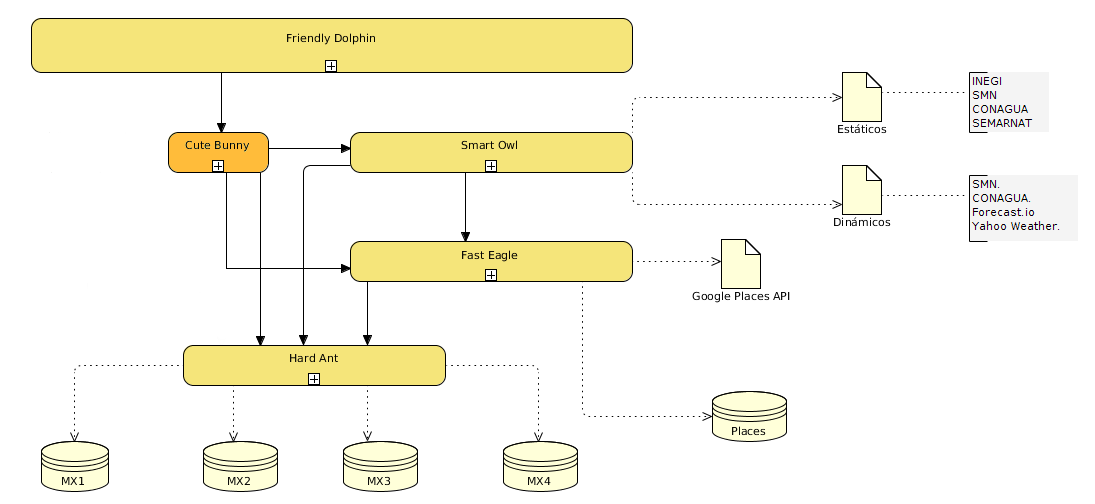
\includegraphics[width=\textwidth]{./images/DiagramaAmbienta2MX_CuteBunny.png}
        \caption{Cute Bunny, Módulo de Ambienta2MX.}
    \end{figure}
    \paragraph{Cute Bunny interactúa con todos módulos de Ambienta2MX, Smart Owl, Hard Ant y Fast Eagle. La interacción con estos surge debido a que Hard Ant es el encargado de gestionar el acceso a las bases de datos de tipo MX y Smart Owl brindará y dará solución a las busquedas que no se encuentren en las bases de tipo MX, es decir, tratará de encontrar la información que Cute Bunny le solicitó para guardarla en algunas de las bases y posteriormente regresar el resultado al solicitante, en el caso de Fast Eagle, para la búsqueda de locaciones en la base de datos Places.}
  \subsection{Alcances}
    \paragraph{Considerando el objetivo primordial, qué es el de comunicar y unir, su único alcance es el de mantener la conexión de forma transparente entre los módulos y permitir la interacción como si todos se encontraran dentro de una misma máquina o servicio único; esto con la finalidad de brindar el acceso a los datos mediante una API de tipo REST libre del contexto y alcance de cada módulo.}
    \paragraph{Considerando la aplicación de un servidor como Nginx, se puede permitir expandir la funcionalidad sin mostrar al usuario la existencia de diversos sistemas trabajando bajo la misma dirección, es una de sus más grandes bondades.}
  \subsection{Restricciones}
    \paragraph{Una de las principales limitantes de éste módulo se ve reflejada en el negocio, debido a que carece de una capa lógica o de procesos entonces se terminó por delegar la información y la lógica a los otros proyectos involucrados.}
    \paragraph{Para éste módulo se decidió hacer uso de un servicio tipo proxy que sólo se encarga de mantener la transparencia como una API única, carece totalmente de un sentido en el negocio y puede ser cambiado por algún otro tipo de servidor web.}
  \subsection{Arquitectura}
    \paragraph{A continuación se mostrará el diagrama por bloques que define la estructura de Cute Bunny.}
      \begin{figure}[b!]
        \centering
        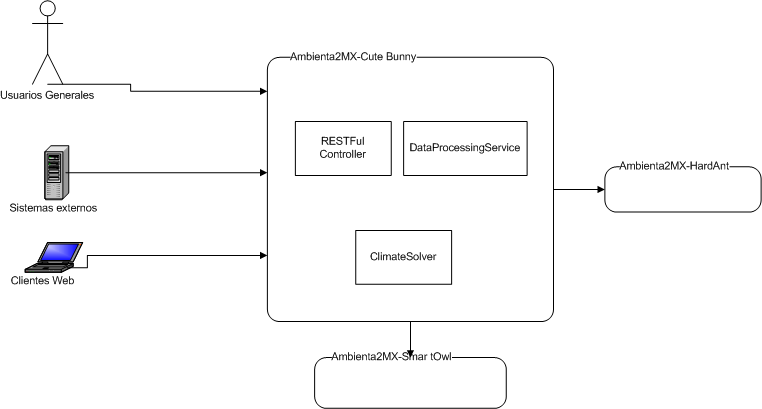
\includegraphics[width=\textwidth]{./images/DiagramaCuteBunny.png}
        \caption{Diagrama General de Cute Bunny}
      \end{figure}
    \paragraph{Como puede ser visualizado, funge como el pegamento de todos los módulos para que éstos puedan ser accedidos desde la vista (Friendly Dolphin), o bien, que servicios de externos puedan alimentarse de la información climatológica obtenida por el sistema Ambienta2MX.}    
  \subsection{Factibilidad}      
    \paragraph{Originalmente se tenía pensado realizar la implementación y unión de todos los módulos del negocio de Ambienta2MX utilizando la tecnología Grails, sin embargo, se dió un cambio drástico debido a que el framework realmente no sería utilizado al 100\%, lo cual nos permitió visualizar el problema desde un punto más de DevOps \cite{38}, optando por la aplicación del servidor nginx como pieza para la unión del sistema.}
    \paragraph{A continuación se muestran las características principales de cada tecnología:}
    \paragraph{``Grails''}    
    \begin{itemize}
      \item Web Framework basado en un patrón MVC.
      \item Trabajo bajo una convención sobre configuración.
      \item Funcionamiento bajo la máquina virtual de Java (JVM)
    \end{itemize}
    \paragraph{``Nginx''}    
    \begin{itemize}
      \item Servidor HTTP orientado a microservicios.
      \item Escrito en C, soporta caché de peticiones y balance de carga.
      \item Soporte para la actualización al protocolo HTTP v2.
    \end{itemize}
    \paragraph{Cómo puede visualizarse, no existe punto de comparación ente ambas tecnologías, este cambio se realizó debido al enfoque se tenía con la aplicación y definición del módulo Cute Bunny desde una instancia inicial. ``Grails'' se encuentra definido como parte de un servidor de aplicación (Tomcat o Jetty), mientras Nginx es un Web Server (Semejante a Apache2).}
    \paragraph{La información del servidor puede ser visualizada con más detalle en el Anexo 6: Instalación y configuració de Nginx.}  